\subsection{Magnetic Anomaly Approximation}
In reality, the Earth's magnetic field \(\Vec{T}\) is always present, and if we assume that there are no sources for magnetic anomalies other than the cable, the sensor records:
\begin{equation*}
    \vec{F_s} = \vec{T} + \vec{B}_s
\end{equation*}

Moreover, in practical situations one typically has \(\vec{B}_s << \vec{T}\), with \(B_s\) on the order of \(\mu\text{T}\). Consequently, \highlight{for a scalar magnetometer \footnote{Practically, the norm of a fluxgate magnetometer is used, for its lower cost, and taking its norm makes it more robust against the noise from trajectory fluctuations and other types of external motion noise.} recording \(F_s\), \(B_s\) can be treated as the projection of \(\vec{B}_s\) onto the unitary vector of the Earth's magnetic field \(\vec{T}\), which is constant during measurements, \cite[Chapter~2, Section~7.2]{nodot:tel-01155714}, see Figure~\ref{fig:ill_anom}.}

\begin{figure}
    \centering
    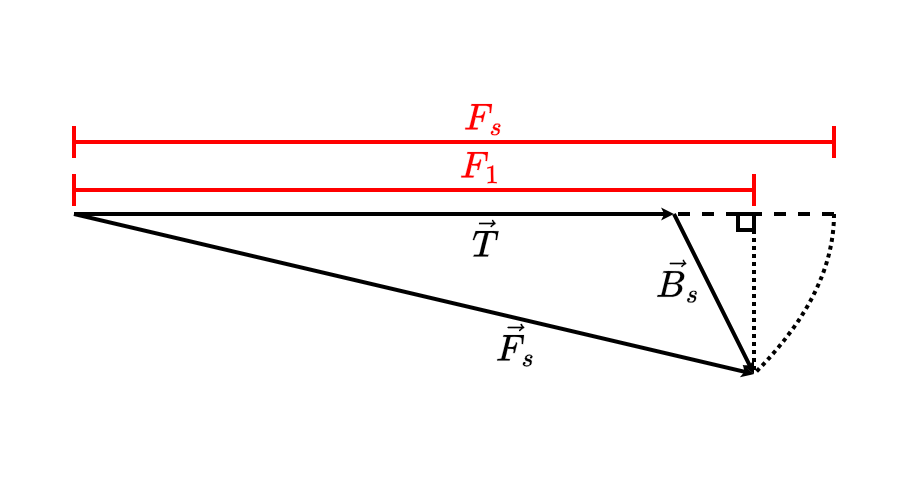
\includegraphics[width=\linewidth]{methodology/figures/anomaly_geometry.png}
    \caption{geometrical illustration of the magnetic anomaly}
    \label{fig:ill_anom}
\end{figure}

thus,
\begin{equation*}
    \lvert \vec{F_s} \lvert \approx F_1 = \lvert\vec{T}\lvert + \frac{\vec{B_s}.\vec{T}}{\lvert\vec{T}\lvert}
\end{equation*}
The magnetic anomaly generated by the cable is approximately:
\begin{equation*}
    S \approx F_1 - \lvert\vec{T}\lvert = \frac{\vec{B_s}.\vec{T}}{\lvert\vec{T}\lvert}
\end{equation*}

To generalize the model, Earth's magnetic field is inclined by \(\delta\), and the CPA reference axis forms an angle \(\psi\) with magnetic north:
{\scriptsize
\begin{equation*}
    S(\tau) = \frac{\mu_0 I}{2 \pi d} 
    \left(
    \begin{pmatrix}
        \cos{\psi} & -\sin{\psi} & 0 \\
        \sin{\psi} & \cos\psi & 0 \\
        0 & 0 & 1
    \end{pmatrix}
    \begin{pmatrix}
        \frac{1}{1+\tau^2} \\ 0 \\ \frac{\tau}{1+\tau^2}
    \end{pmatrix}
    \right)
    \cdot
    \begin{pmatrix}
        \cos\delta \\ 0 \\ \sin\delta
    \end{pmatrix}
\end{equation*}
}

Developing and refactoring the previous equation gives:

\begin{equation}
\begin{aligned}
S(\tau) &= K_p \cdot \cos\psi \cdot \cos\delta \cdot \frac{1}{1+\tau^2} 
        + K_p \cdot \sin\delta \cdot \frac{\tau}{1+\tau^2} \\
K_p &=  \frac{\mu_0 I}{2 \pi d}.
\end{aligned}
\label{eq:anomaly}
\end{equation}